
\section{Simulation}\label{sec:simulation}
There are four main challenges when we are doing pose and torque control of an object. 
\paragraph{Pure torque control} 
Suppose we have a pivot that avoids the object to translate while it is still able to move and have angular velocity like a door. If there was only one robot touching the obstacle, the ending points of the obstacle was the best location due to Eq. \ref{eq:torque} where $r$ would be maximum and the maximum torque has been created with the same force. But, when there is a swarm of robots, because of its dynamic state it is not true. If the swarm hit the object with mean position at the top, lots of its robots is missed and will make the swarm apart, and also because there remain less robots, force is significantly decreased and torque would not maximize. In our simulation, the swarm will try to make torque as much as possible until it is passed the object, when it is passed, it will gather itself in one corner which is very time consuming. Fig. \ref{fig:LFig} illustrates how different positions of the object cause different times. 
%When there is only one robot that applies force to an object, the greatest torque is when it apply force to the end of the object. 

\begin{figure}
\begin{center}
	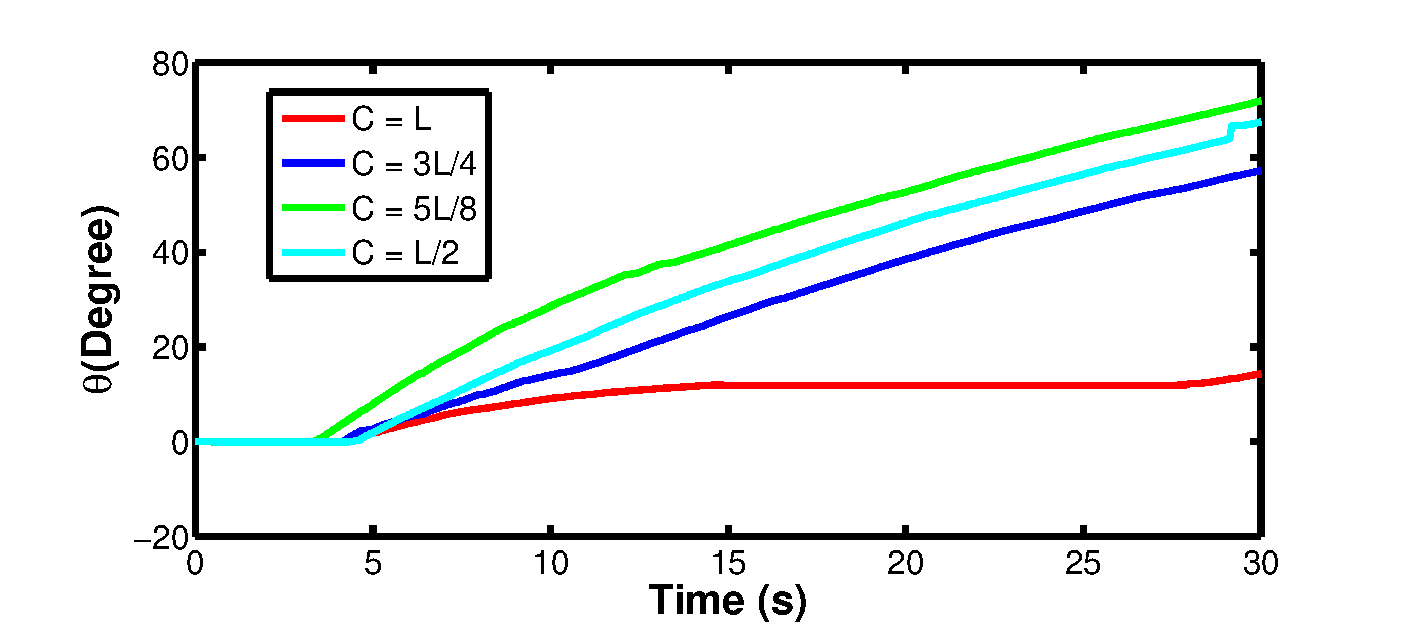
\includegraphics[width=\columnwidth]{LFig.eps}
\end{center}
\vspace{-1em}
\caption{\label{fig:LFig}
Plot showing how changing the mean position of the swarm on the object may affect getting the highest torque and force with 144 robots with a standard deviation of less than $1.5 m$ and the object length of $6m$.
}
\vspace{-1em}
\end{figure}
\paragraph{Pure translation of the object}
In our simulations we used a big uniform density rectangle as object. If the force is applied perpendicular to the object and in line of the center of mass, according to Eq. \ref{eq:torque} there would be no torque. We proposed the following goal position for mean position of the swarm in which uses the difference between the goal angle and the current object angle, $\Delta \theta$ to find where to apply force, $C$ is a constant and $O_x,O_y$ is the object COM position.
\begin{align}\nonumber
goal_y &= C \Delta \theta + O_y\\
goal_x &= O_x
\end{align}

We use a PD controller to control mean position as in \cite{ShahrokhiIROS2015}. Fig. \ref{fig:PosControlFig} shows how $\Delta \theta$ converges to zero with different locations of the swarm. When it is upper or downer of the object, when it hits it makes a little torque but then it tries to cancel it.
\begin{figure}
\begin{center}
	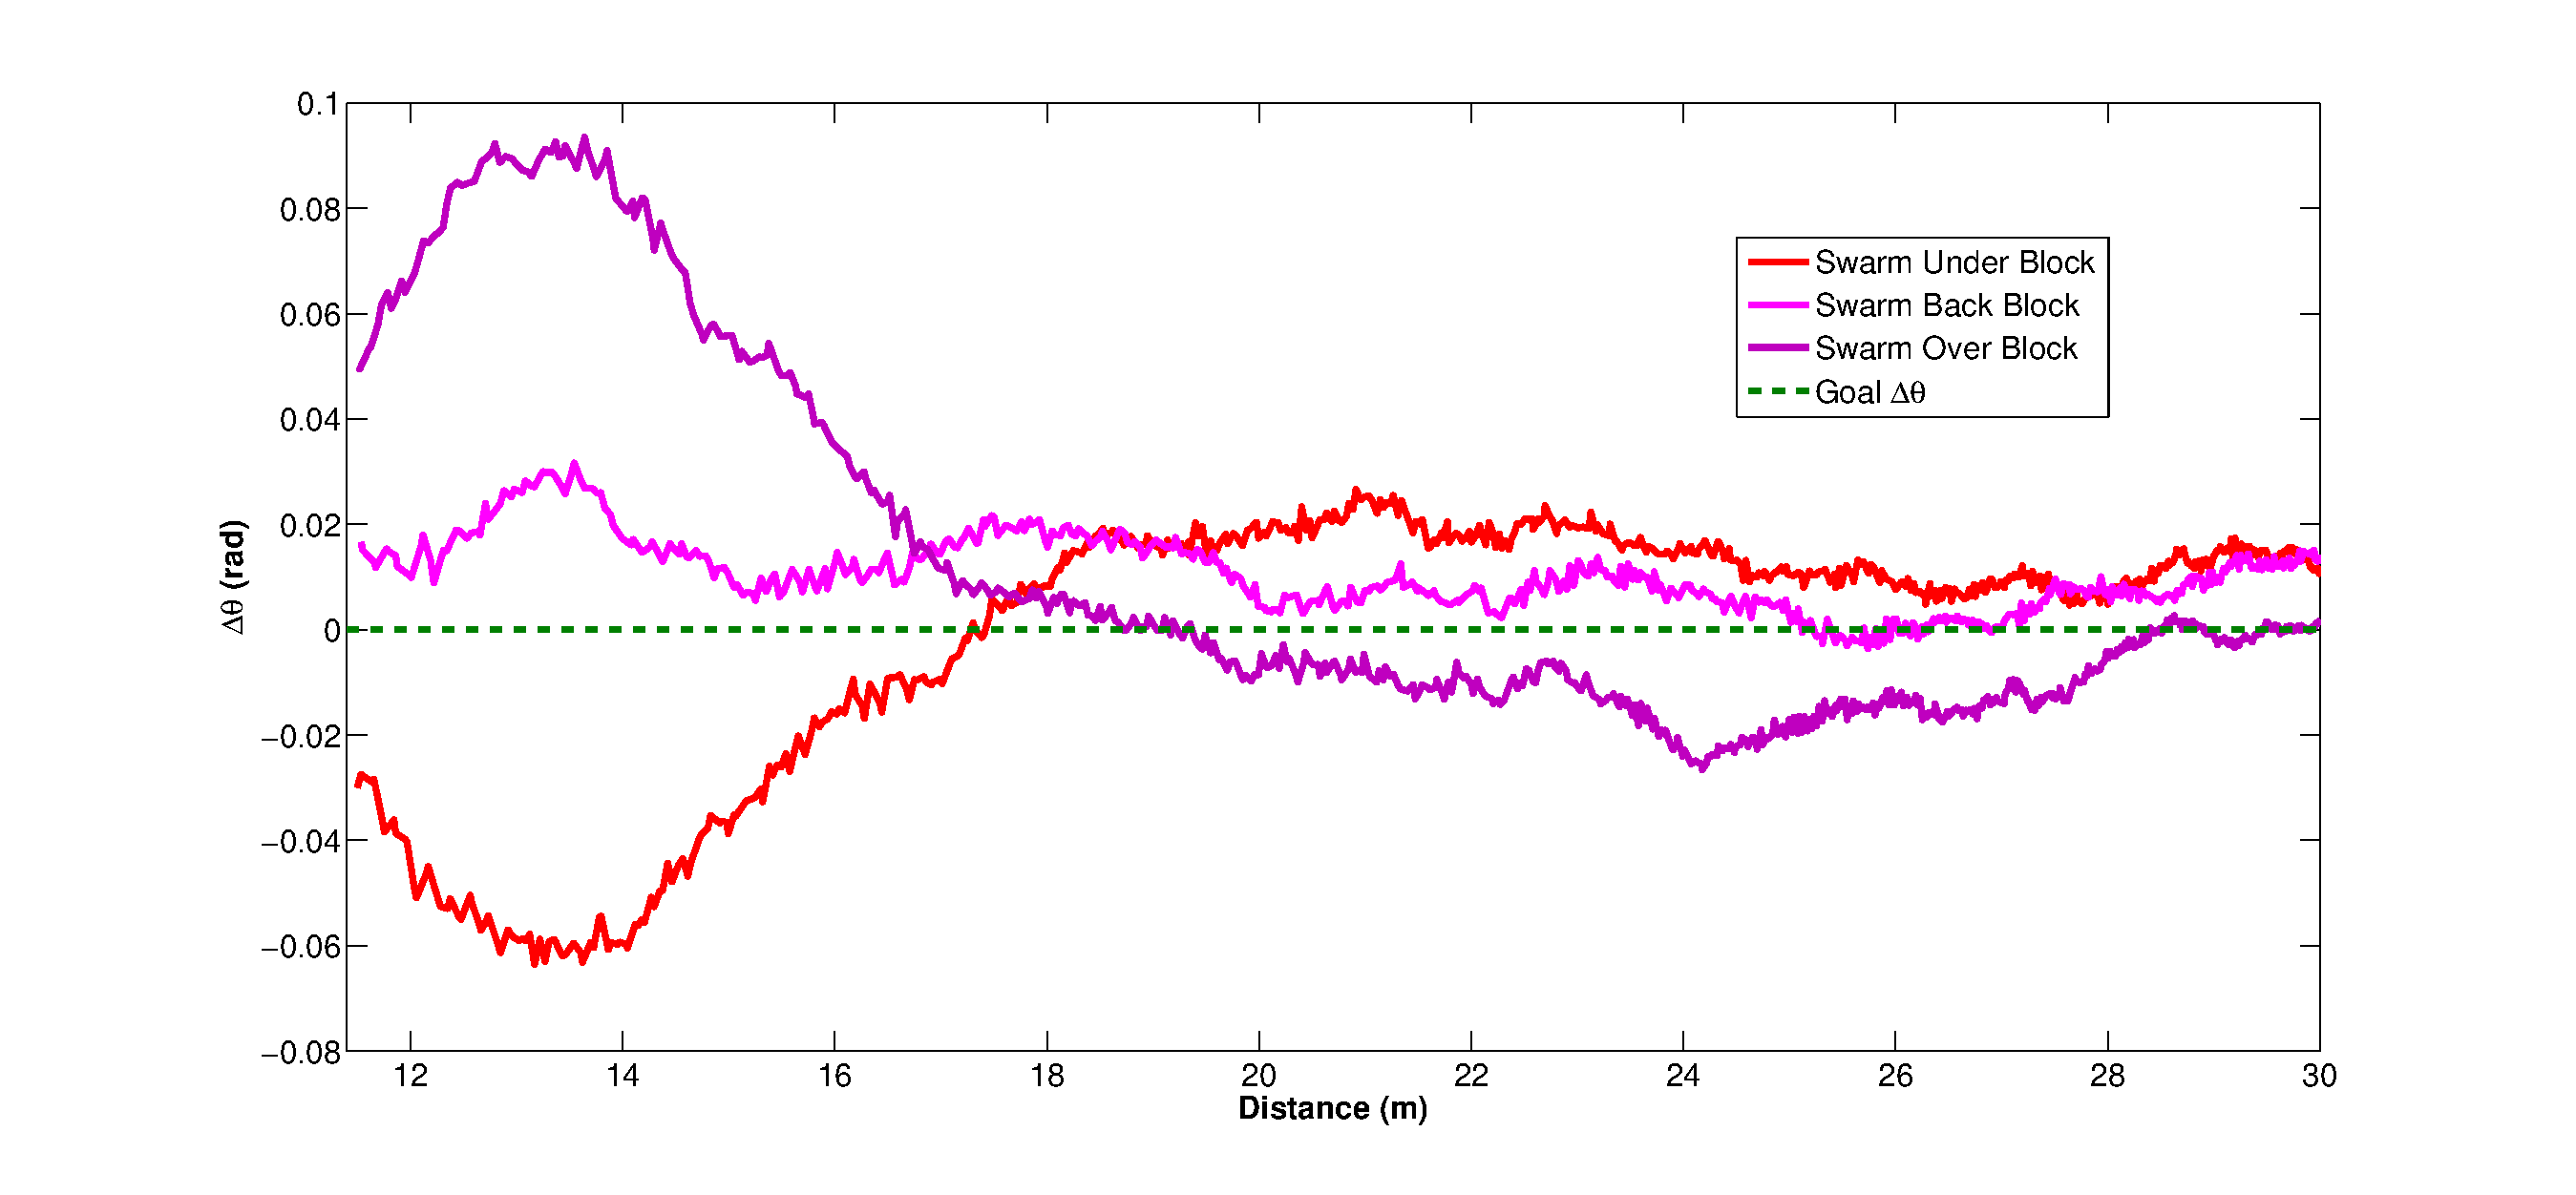
\includegraphics[width=\columnwidth]{PosControlFig.eps}
\end{center}
\vspace{-1em}
\caption{\label{fig:PosControlFig}
The swarm can navigate the object without changing its orientation significantly if it hits in the line of COM of the object and perpendicular to it. It will correct itself if it makes some torque.
}
\vspace{-1em}
\end{figure}

\paragraph{Orientation of the object}
Using the pure torque control that we discussed, we can control the orientation of the object with applying force to it. We do not have pivot here so the rectangle would move besides rotating. We used that data to pick up a more rational length to lead the swarm to hit that spot. However, the swarm still may split and get apart. We use our hysteresis variance control to gather the swarm together again when it is split. The goal position is related to the angle that the object has made already. It should be somewhere upper or downer the COM, inside the object. In the following equation, $O_{\theta}$ is the orientation of the object and $w$ is the width of the object.
\begin{align}\nonumber
goal_y &= O_y + 0.66cos(O_{\theta})w\\
goal_x &= O_x + 0.66sin(O_{\theta})w
\end{align}
Fig. \ref{fig:OrientCont} illustrates this controller with different starting positions. When the lines are steady, it means that the variance had grown more and the swarm was on variance control mode.
\begin{figure}
\begin{center}
	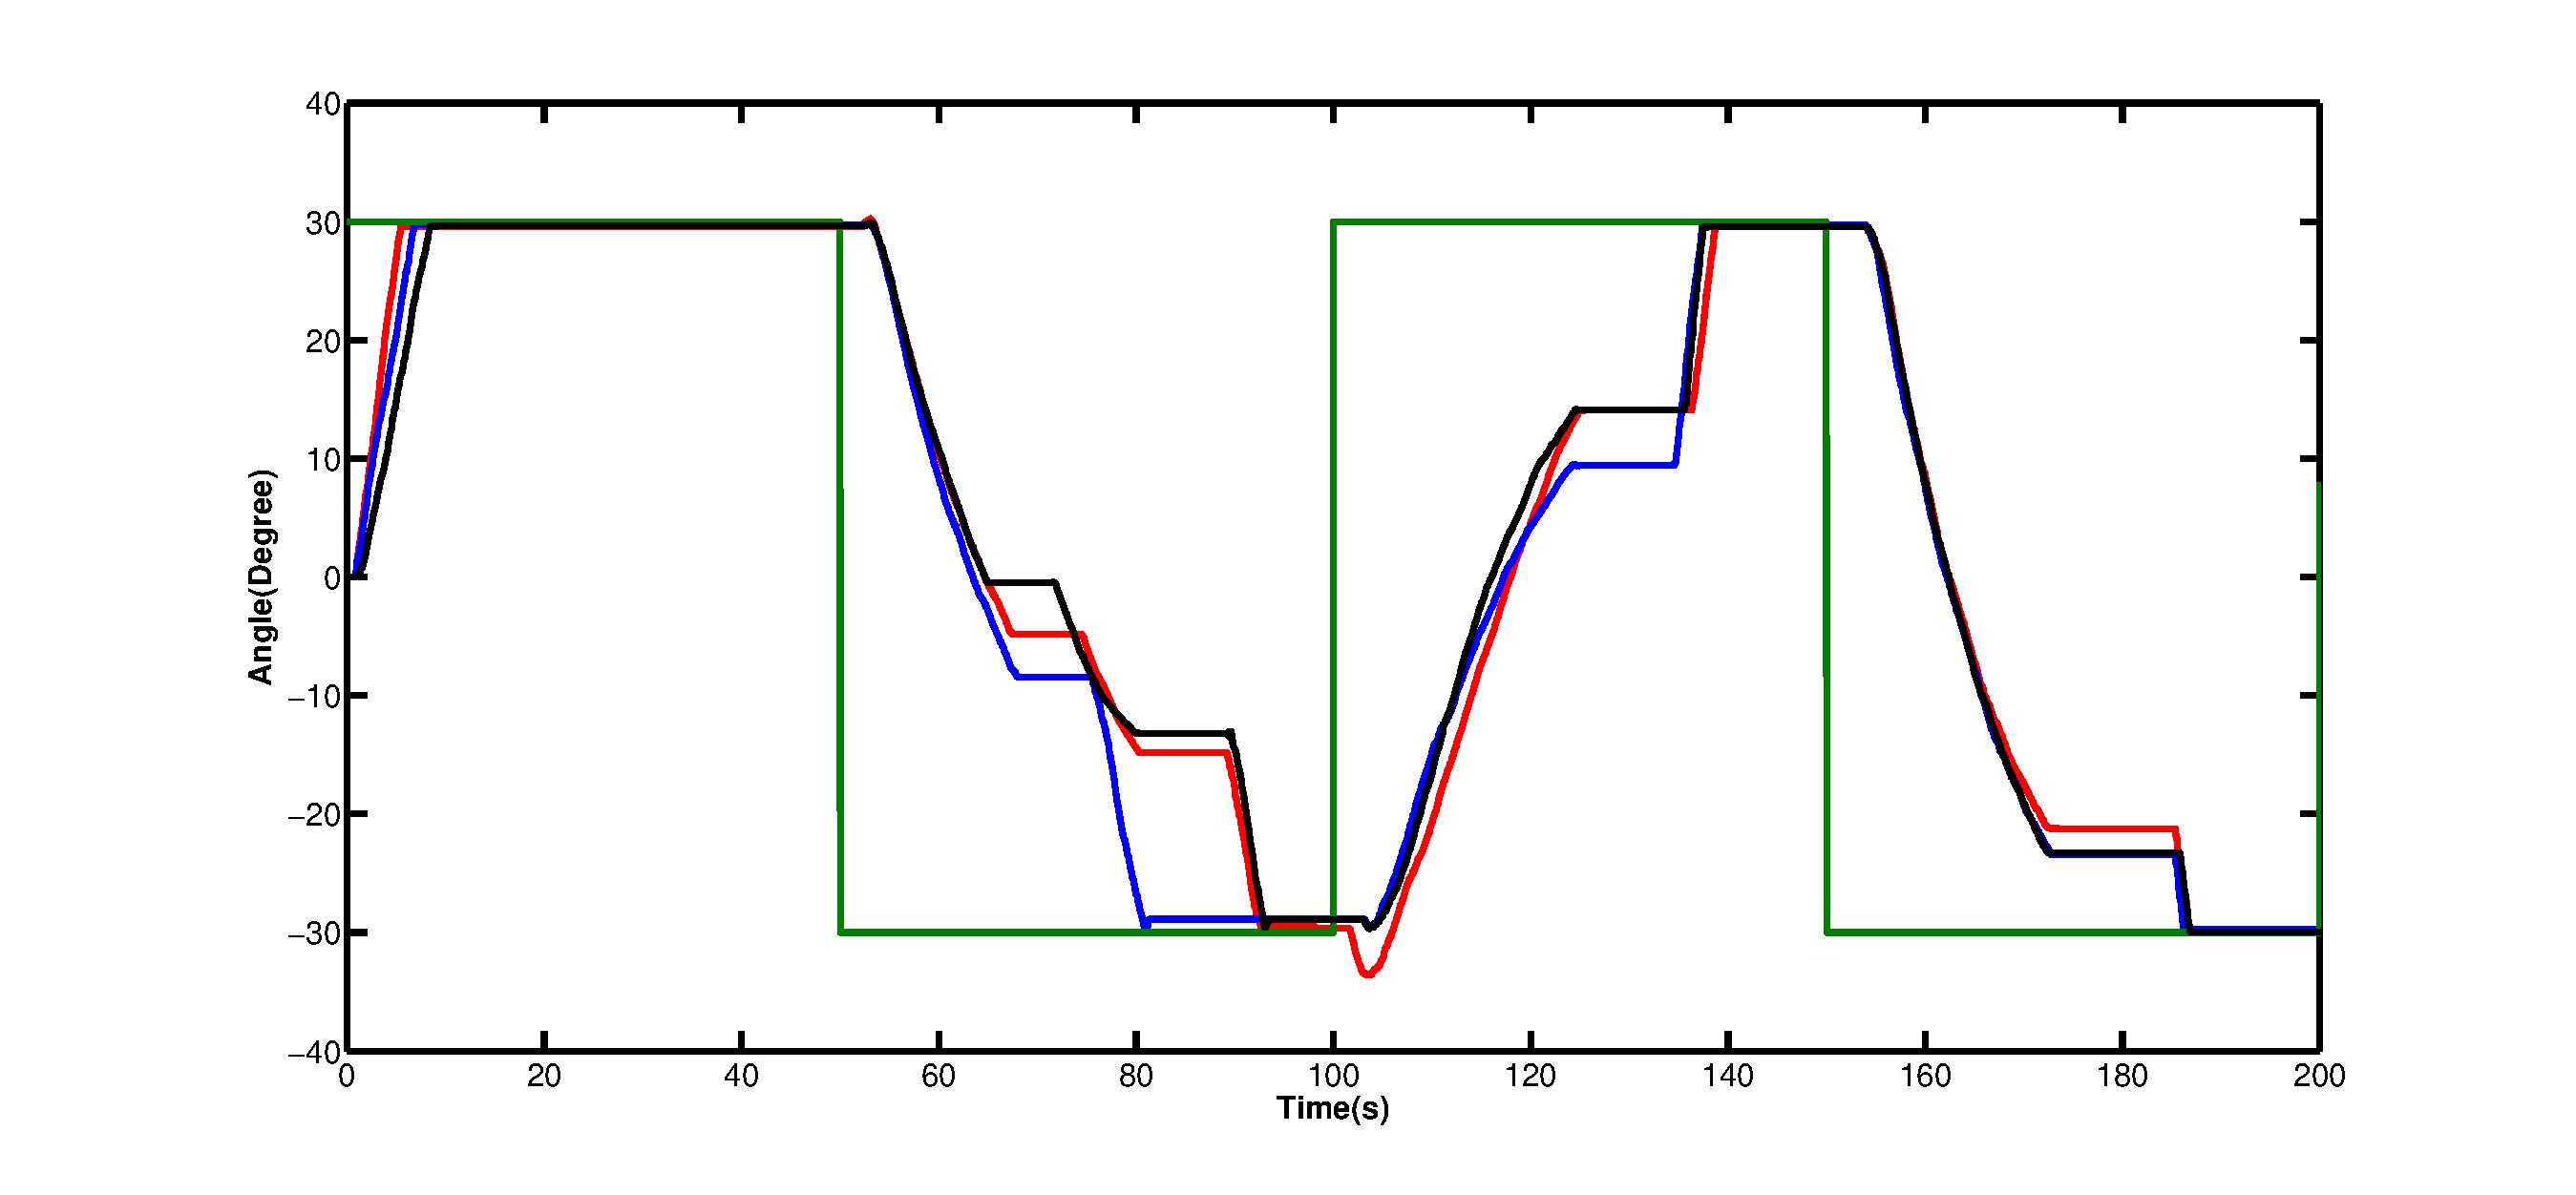
\includegraphics[width=\columnwidth]{OrientationContFig.eps}
\end{center}
\vspace{-1em}
\caption{\label{fig:OrientCont}
This plot shows how we can control orientation of the object. The green line is the goal orientation, at the times that other lines are steady, it is because the swarm is on variance control mode.
}
\vspace{-1em}
\end{figure}


